\documentclass[11pt, a4paper]{article}
\usepackage[utf8]{inputenc}

\usepackage[margin=1in]{geometry} 
\usepackage{amsmath,amsthm,amssymb}
\usepackage[margin=1in]{geometry} 
\usepackage{amsmath,amsthm,amssymb}

\usepackage[slovene]{babel}
\usepackage{color}
\usepackage{graphicx}
\usepackage{amssymb}
\usepackage{amsmath}
\usepackage{mathtools}
\usepackage{commath}
\usepackage{ragged2e}
\usepackage[T1]{fontenc}
\usepackage[normalem]{ulem}
\usepackage{amsthm}
\usepackage{esvect}
\usepackage{float}
\usepackage{calrsfs}
\DeclareMathAlphabet{\pazocal}{OMS}{zplm}{m}{n}
\newcommand{\Ga}{\mathcal{G}}
\mathtoolsset{showonlyrefs} 

\newcommand\setItemnumber[1]{\setcounter{enumi}{\numexpr#1-1\relax}}


\newtheorem{theorem}{Trditev}[section]
\newtheorem{corollary}{Posledica}[section]
\newtheorem{lemma}[section]{Lema}
\theoremstyle{definition}
\newtheorem{definition}{Definicija}[section]
\theoremstyle{example}
\newtheorem{example}[section]{Primer}
\theoremstyle{izrek}
\newtheorem{izrek}[section]{Izrek}

\begin{document}
\begin{center}
\thispagestyle{empty}
\parskip=14pt%
\vspace*{3\parskip}%
\begin{Huge} Franck-Hertzov poskus\end{Huge}

By

Matic Tonin

ID No. (28181098)

Mentor 

(Rok Dolenec)

\rule{7cm}{0.4pt}

Pod okvirom:

FAKULTETE ZA FIZIKO IN MATEMATIKO, LJUBLJANA

17. 4. 2020

\end{center}
\pagebreak
\section{Naloga}
\begin{enumerate}
\item Opazuj odvisnost toka $I_2$ med anodno mrežico in anodnim kolektorjem v odvisnosti od negativne napetost $U_1$ na katodi. Spreminjaj temperaturo in posebej natančno opazuj in izmeri položaje vseh vrhov v merjenih odvisnostih. Skiciraj odvisnosti pri petih različnih temperaturah, ko se slike primerno razlikujejo, to je približno pri temperaturah okoli 180, 160, 140 in 120 C in na koncu še pri sobni temperaturi.
\item  Natančno določi položaje vrhov $U_1$, $n = U_2+n \Delta \frac{E}{e_0}$ pri posameznih temperaturah in rezultate vnesi v tabelo. Razlike napetosti med zaporednimi maksimumi ustrezajo energiji, ki jo izgubijo elektroni pri posameznem neelastičnem trku z atomom Hg. Določi $\Delta E= E_1-E_0$ $= e_0 \Delta U_1$, kjer sta $E_1$ in $E_0$ energiji prvega vzbujenega in osnovnega stanja elektrona v zunanji lupini Hg.
\end{enumerate}

\section{Postopek dela}
Najprej postavimo vezavo, kot napovedjejo prednavodila. Tok $I_2$ pretvorimo v napetostni signal, ki ga bomo zaznavali na osciloskopu in sicer z enačbo:

$$U_{sig}=\eta I_2 R \quad R= 1 M\Omega$$
Negativno napetost $U_1$ pa pošljemo na X-vhod osciloskopa. 
Osciloskop nastavimo, kot piše v navodilih. Vedeti moramo, da sta obe napetosti negativni, zato za lažje delo invertiramo Y os z opcijo na osciloskopu. Pojavilo pa se bo tudi veliko šuma, ki pride zaradi motenj pri frekvenci 50 HZ. Cev egrejemo do začetne temperature merjenja, torej 180 °C in tam, zaradi manjšega šuma izklopimo grenlik ter prižgemo ventilator. Potem približno na vsakih 20 °C skiciramo signal, ter razberemo razdalje med max amplitudami. Na koncu celico ohladimo na temperature ozračja in izmerimo odvisnost tudi takrat.
 
\pagebreak
\section{Meritve}
V našem primeru smo merili pri temperaturah 180, 160, 140, 120 °C, zato si bomo pogledali vsako posebej in vrednosti zapisali v tabelo. 
\subsection{Temperatura 180 °C}
Pri temperaturi 180 °C naredimo sliko na osciloskopu in jo nato obdelujemo. Slika je: 

\begin{figure}[H]
    \centering
    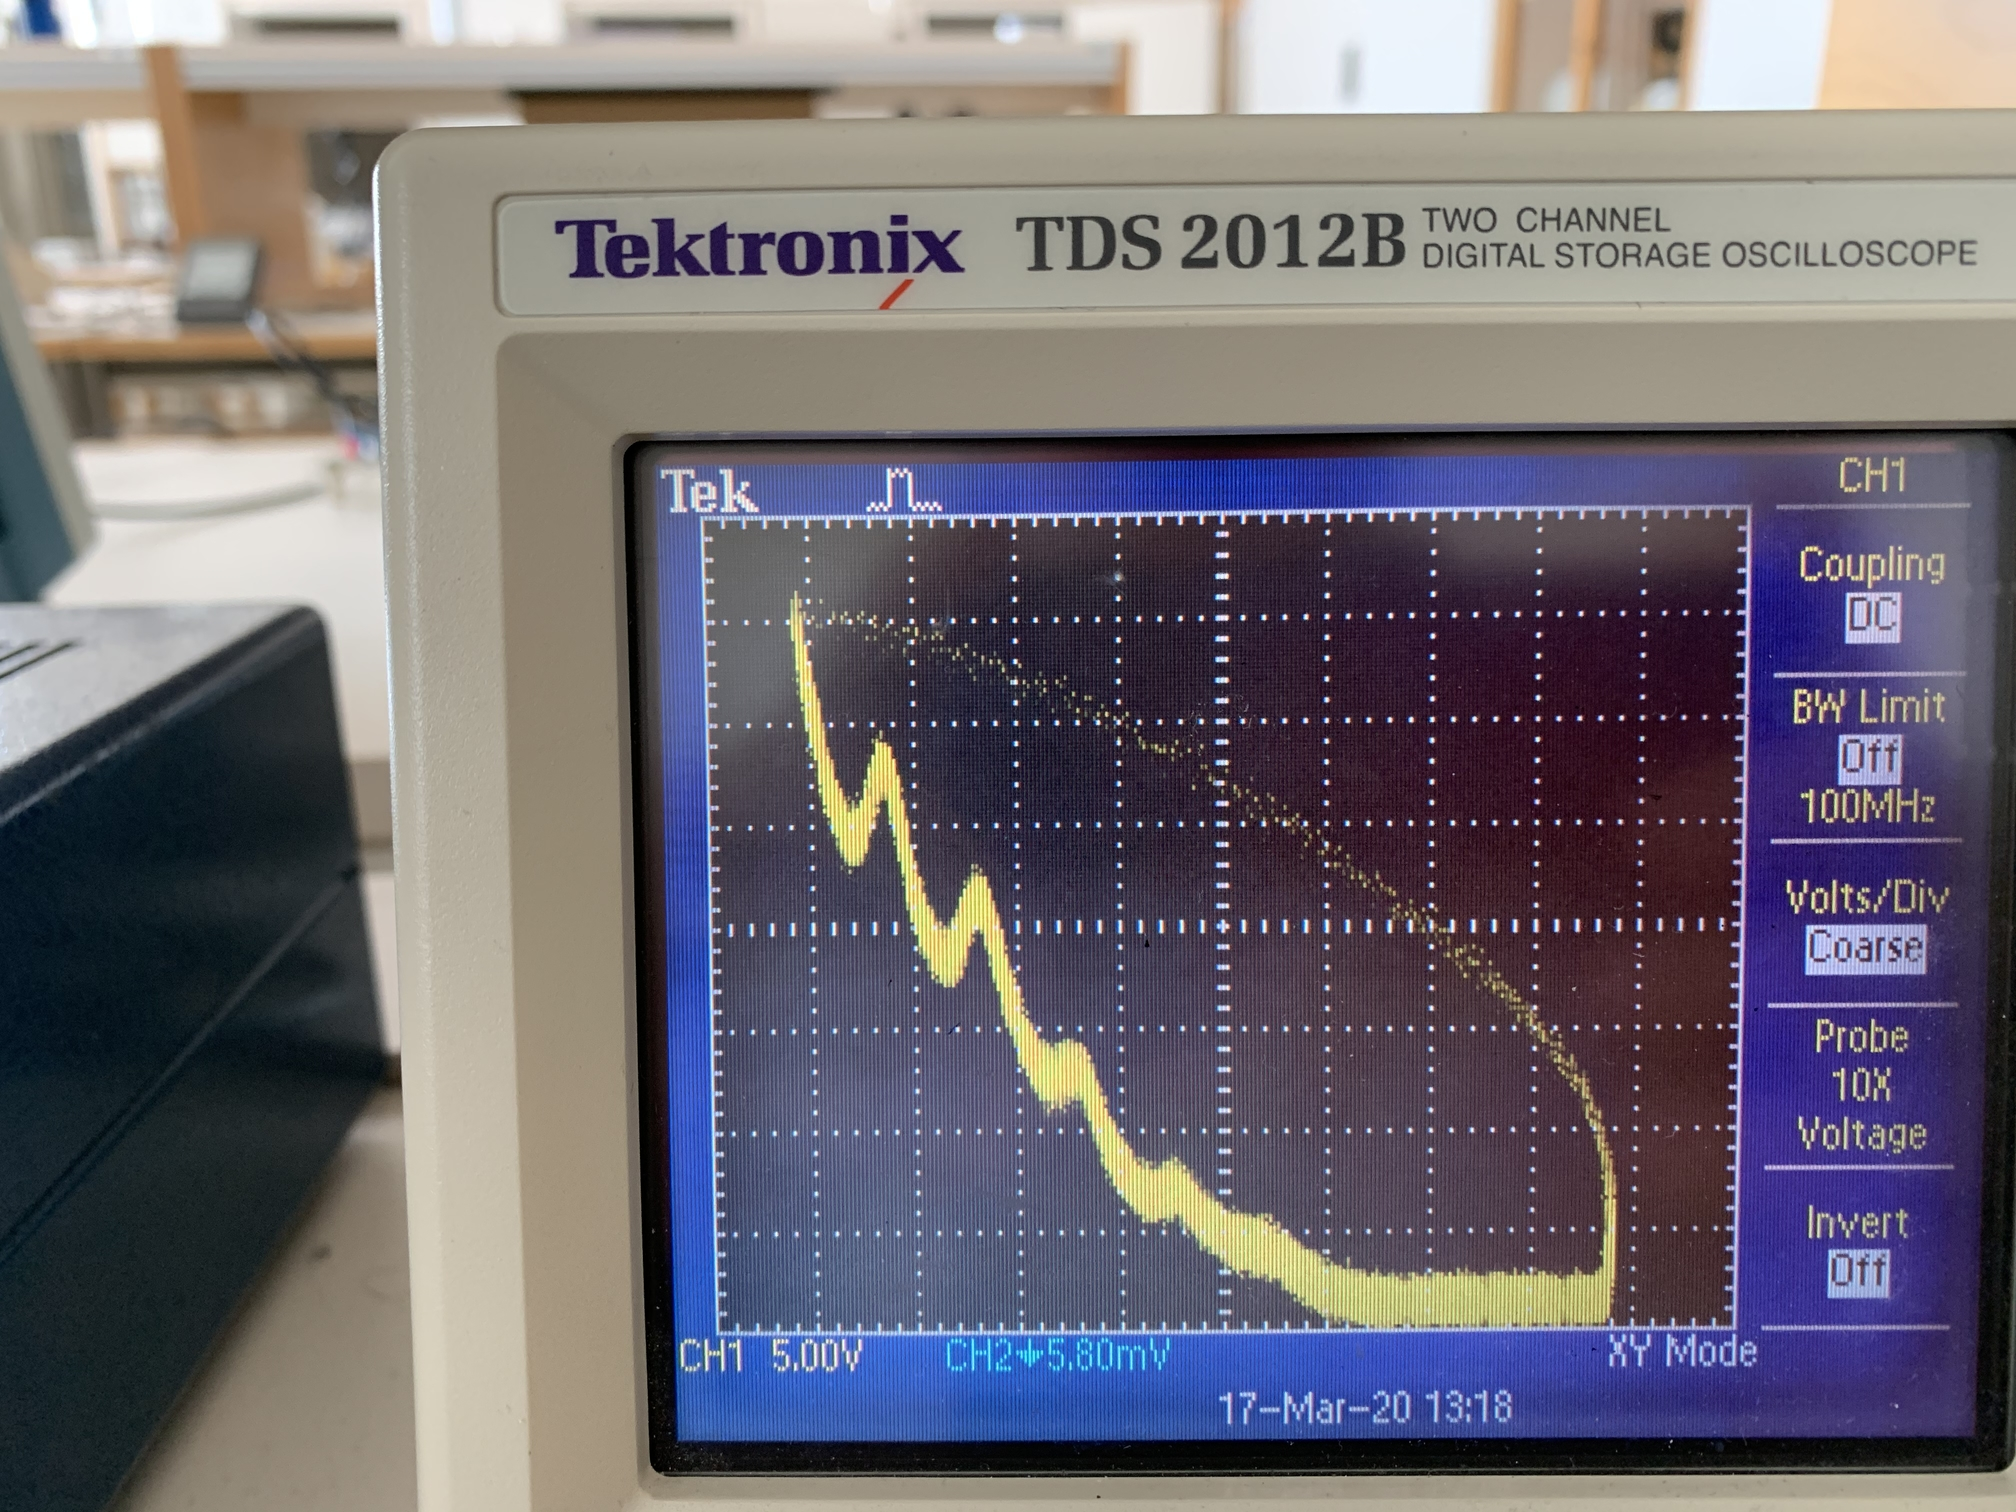
\includegraphics[width=10cm]{T=180_max_napetost.jpg}
    \caption{Prikaz spreminjanja $U_2$ in $U_{sig}$ na osciloskopu, 180 °C}
\end{figure}
Na x osi imamo prikazano negativno napetost $U_1$ na y osi pa je prikazana napetost signala $U_{sig}=\eta I_2 R.$
V uvodu zvemo, da je $U_1$ naša pospečevalna napetost elektronov proti anodni mrežici, $I_2$ pa je tok elektronov, ki uspe doseči anodni kolektor. Ker pa v naši celici imamo še atome Hg, te elektroni prožno trčijo v atome Hg in pri dovolj veliki kinetični energiji elektrona, ki jo zgeneriramo z $U_1$, se lahko zgodi, da elektron po neprožnem trku z atomom Hg, ga vzbudi v prvo vzbujeno stanje. To lahko zapišemo z enačbo: 


$$U_1=\frac{\Delta E}{e_0}$$

Po nadaljnem večanju, se zgodi, da drug elektron trči atom Hg in se ponovno zgdoi padec napetosti na signalu $I_2$. In to se dobro vidi na naši sliki. Vidimo periodično ponavljanje razmikov maksimumov, ki jih zapišemo v tabelo: 

\begin{table}[h]
	\centering
	\begin{tabular}{|c|c|c|c|c|c|}
		\hline
		
		Številka vrha & $U_1$& $U_2$ & $\Delta U = U_{n}- U_{n-1}$ [V] & $\Delta E= e_0\Delta U $ [eV] & $\overline{\Delta E}$\\
		\hline
		\hline
		1 & 0 & 35 & 0 & 0 & //\\
		\hline
		2 & 3.7 & 29 & 3.7 & 3.7 &// \\
		\hline
		3 & 8.2 & 23 & 4.5 & 4.5 & //\\
		\hline
		4 & 12.8 & 14 & 4.6 & 4.6 & //\\
		\hline
		5 & 17.5 & 7.8 &4.7 & 4.7 &//\\
		\hline
		6 & 22.3 & 6.2 & 4.8 & 4.8 & //\\
		\hline
		//& //& //&// & $4.56 eV \pm 0.25 eV$\\ 
		\hline
		\hline
	\end{tabular}
	\caption{Podatki o vrhovih na naši sliki 1.}		\label{180 °C}
\end{table}
Kometar k tabeli. Prve vrednosti nismo šteli v povprečje, saj je bil to odmik od začetka grafa, oz od začetka prikaza osciloskopa. \\
Vidimo, da je povprečje enako: 

$$\overline{\Delta E}=4.56 eV \pm 0.25 eV$$

Za napako smo ocelili, da je kar 0.25 eV, saj se pojavi zgolj zaradi našega nenatančnega odčitavanja iz grafa. 
\subsection{Temperatura 160 °C}
Pri temperaturi 160 °C naredimo sliko na osciloskopu in jo nato obdelujemo. Slika je: 

\begin{figure}[H]
    \centering
    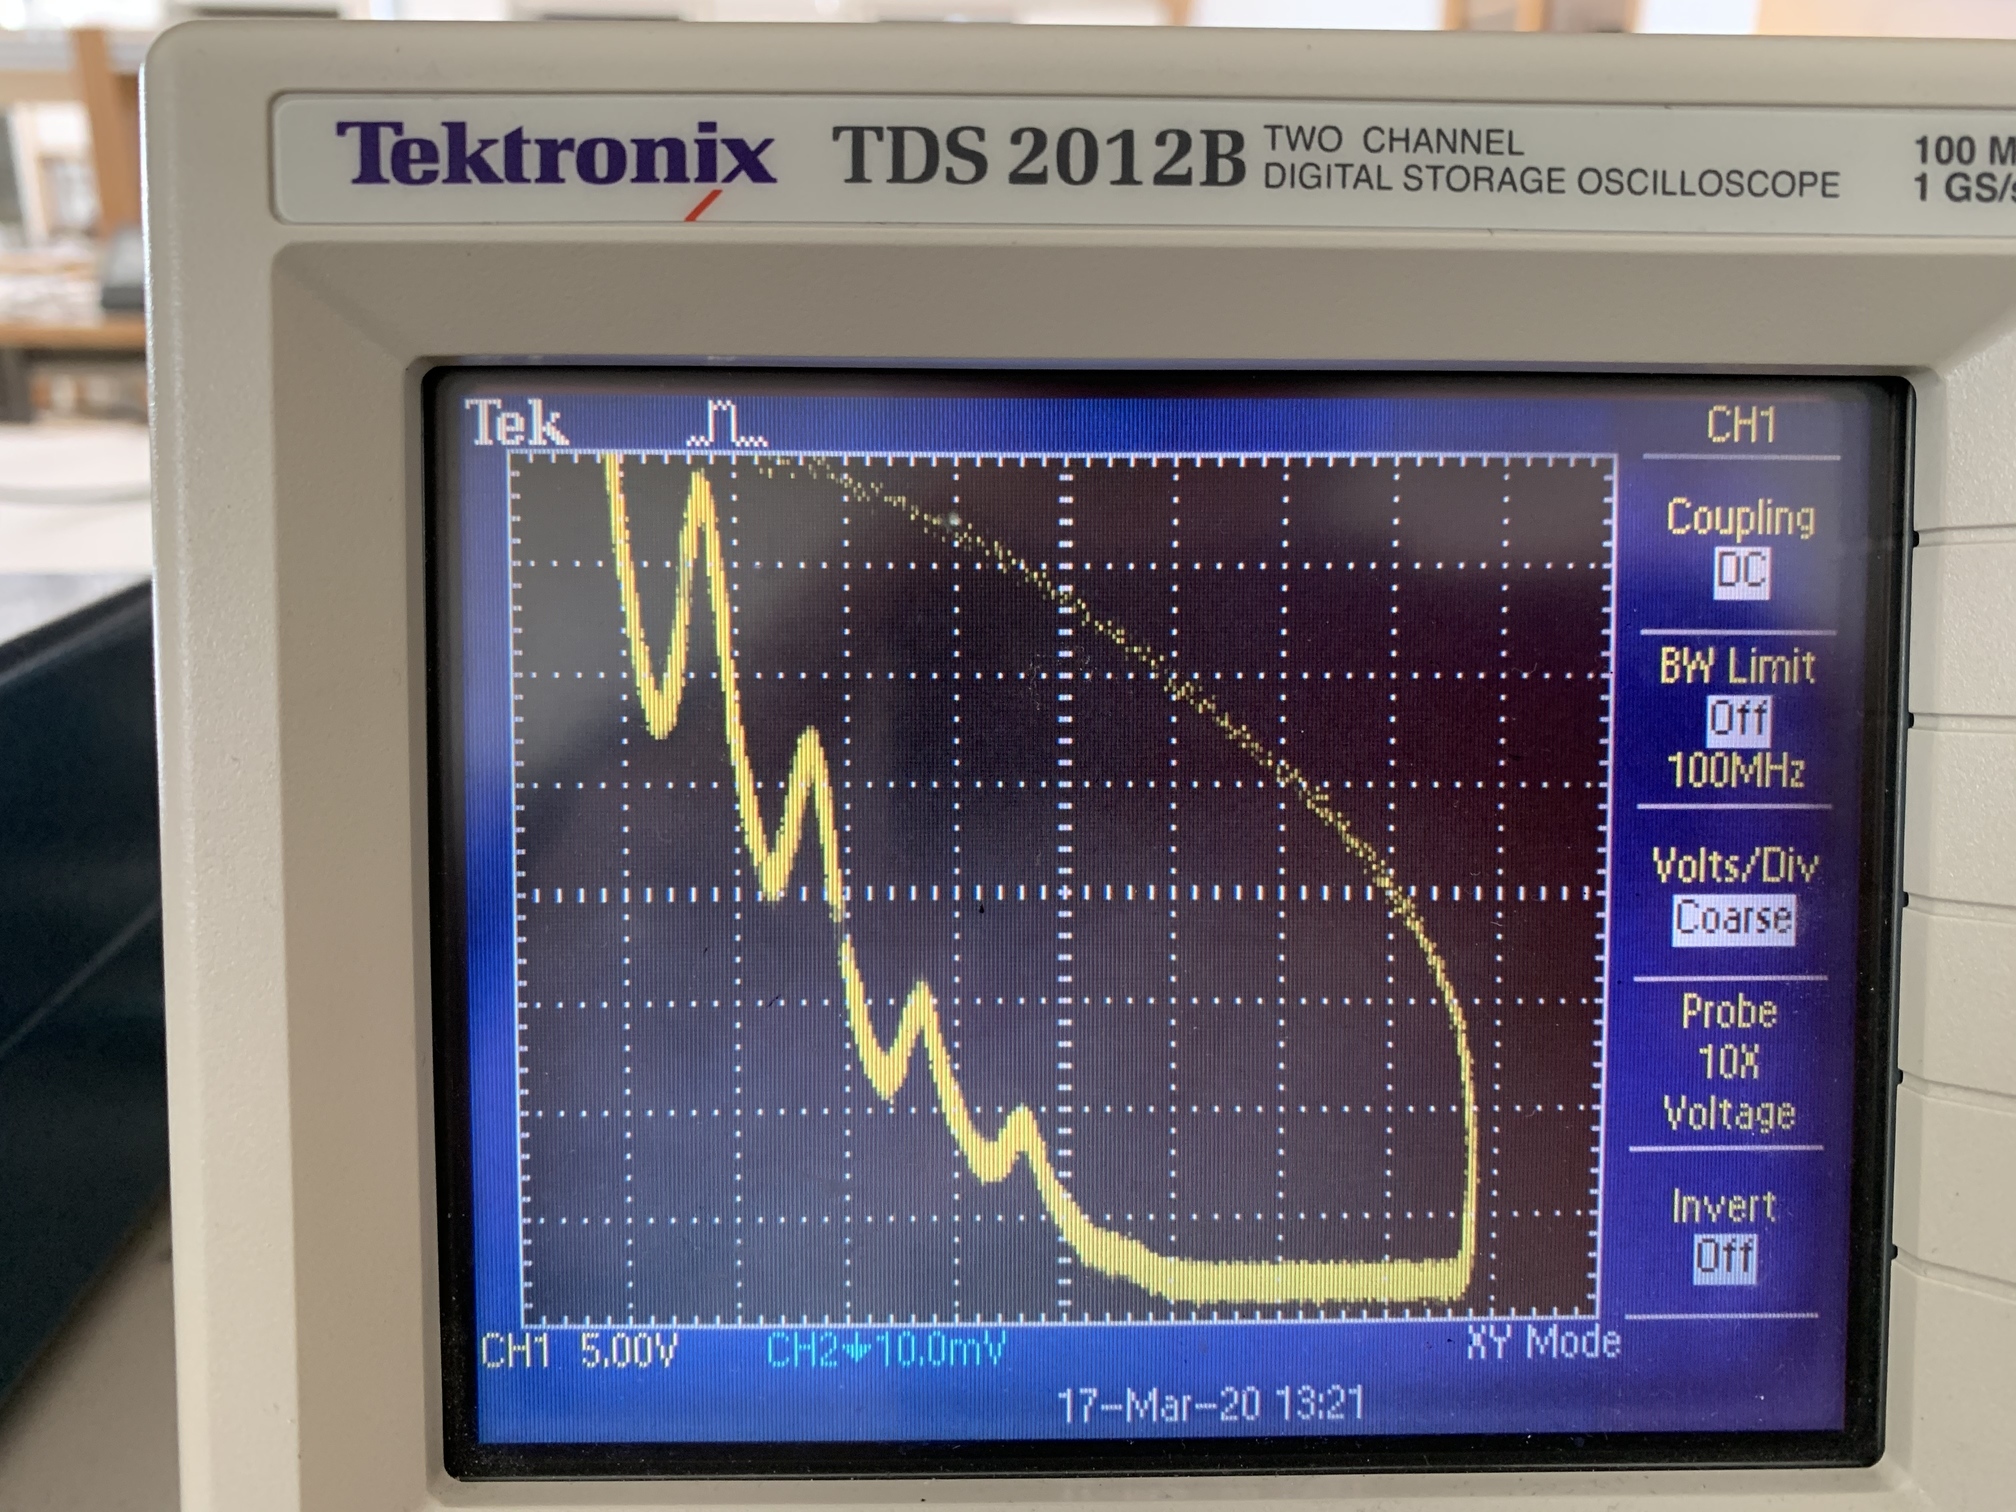
\includegraphics[width=10cm]{T=160_max_napetost.jpg}
    \caption{Prikaz spreminjanja $U_2$ in $U_{sig}$ na osciloskopu, 160 °C}
\end{figure}
Na x osi imamo prikazano negativno napetost $U_1$ na y osi pa je prikazana napetost signala $U_{sig}=\eta I_2 R.$

Če ponovno naredimo tabelo: 
\begin{table}[h]
	\centering
	\begin{tabular}{|c|c|c|c|c|c|}
		\hline
		
		Številka vrha & $U_1$ & $U_2$ & $\Delta U = U_{n}- U_{n-1}$ [V] & $\Delta E= e_0\Delta U $ [eV] & $\overline{\Delta E}$\\
		\hline
		\hline
		1 & 0 & 0 & 0 & //\\
		\hline
		2 & 3.7 & 39 & 3.7 & 3.7 &// \\
		\hline
		3 & 8.3 & 27 & 4.6 & 4.6 & //\\
		\hline
		4 & 13.5 & 16 & 5.2 & 5.2 & //\\
		\hline
		5 & 18 & 10 & 4.5 & 4.5 &//\\
		\hline
		6 & 22.6 & 4 & 4.6 & 4.6 & //\\
		\hline
		//& //& //&// & $4.725 eV \pm 0.25 eV$\\ 
		\hline
		\hline
	\end{tabular}
	\caption{Podatki o vrhovih na naši sliki 2.}		\label{160 °C}
\end{table}
Kometar k tabeli. Prve vrednosti nismo šteli v povprečje, saj je bil to odmik od začetka grafa, oz od začetka prikaza osciloskopa. \\
Vidimo, da je povprečje enako: 

$$\overline{\Delta E}=4.725 eV \pm 0.25 eV$$

Za napako smo ocelili, da je kar 0.25 eV, saj se pojavi zgolj zaradi našega nenatančnega odčitavanja iz grafa.

\subsection{Temperatura 140 °C}
Pri temperaturi 140 °C naredimo sliko na osciloskopu in jo nato obdelujemo. Slika je: 

\begin{figure}[H]
    \centering
    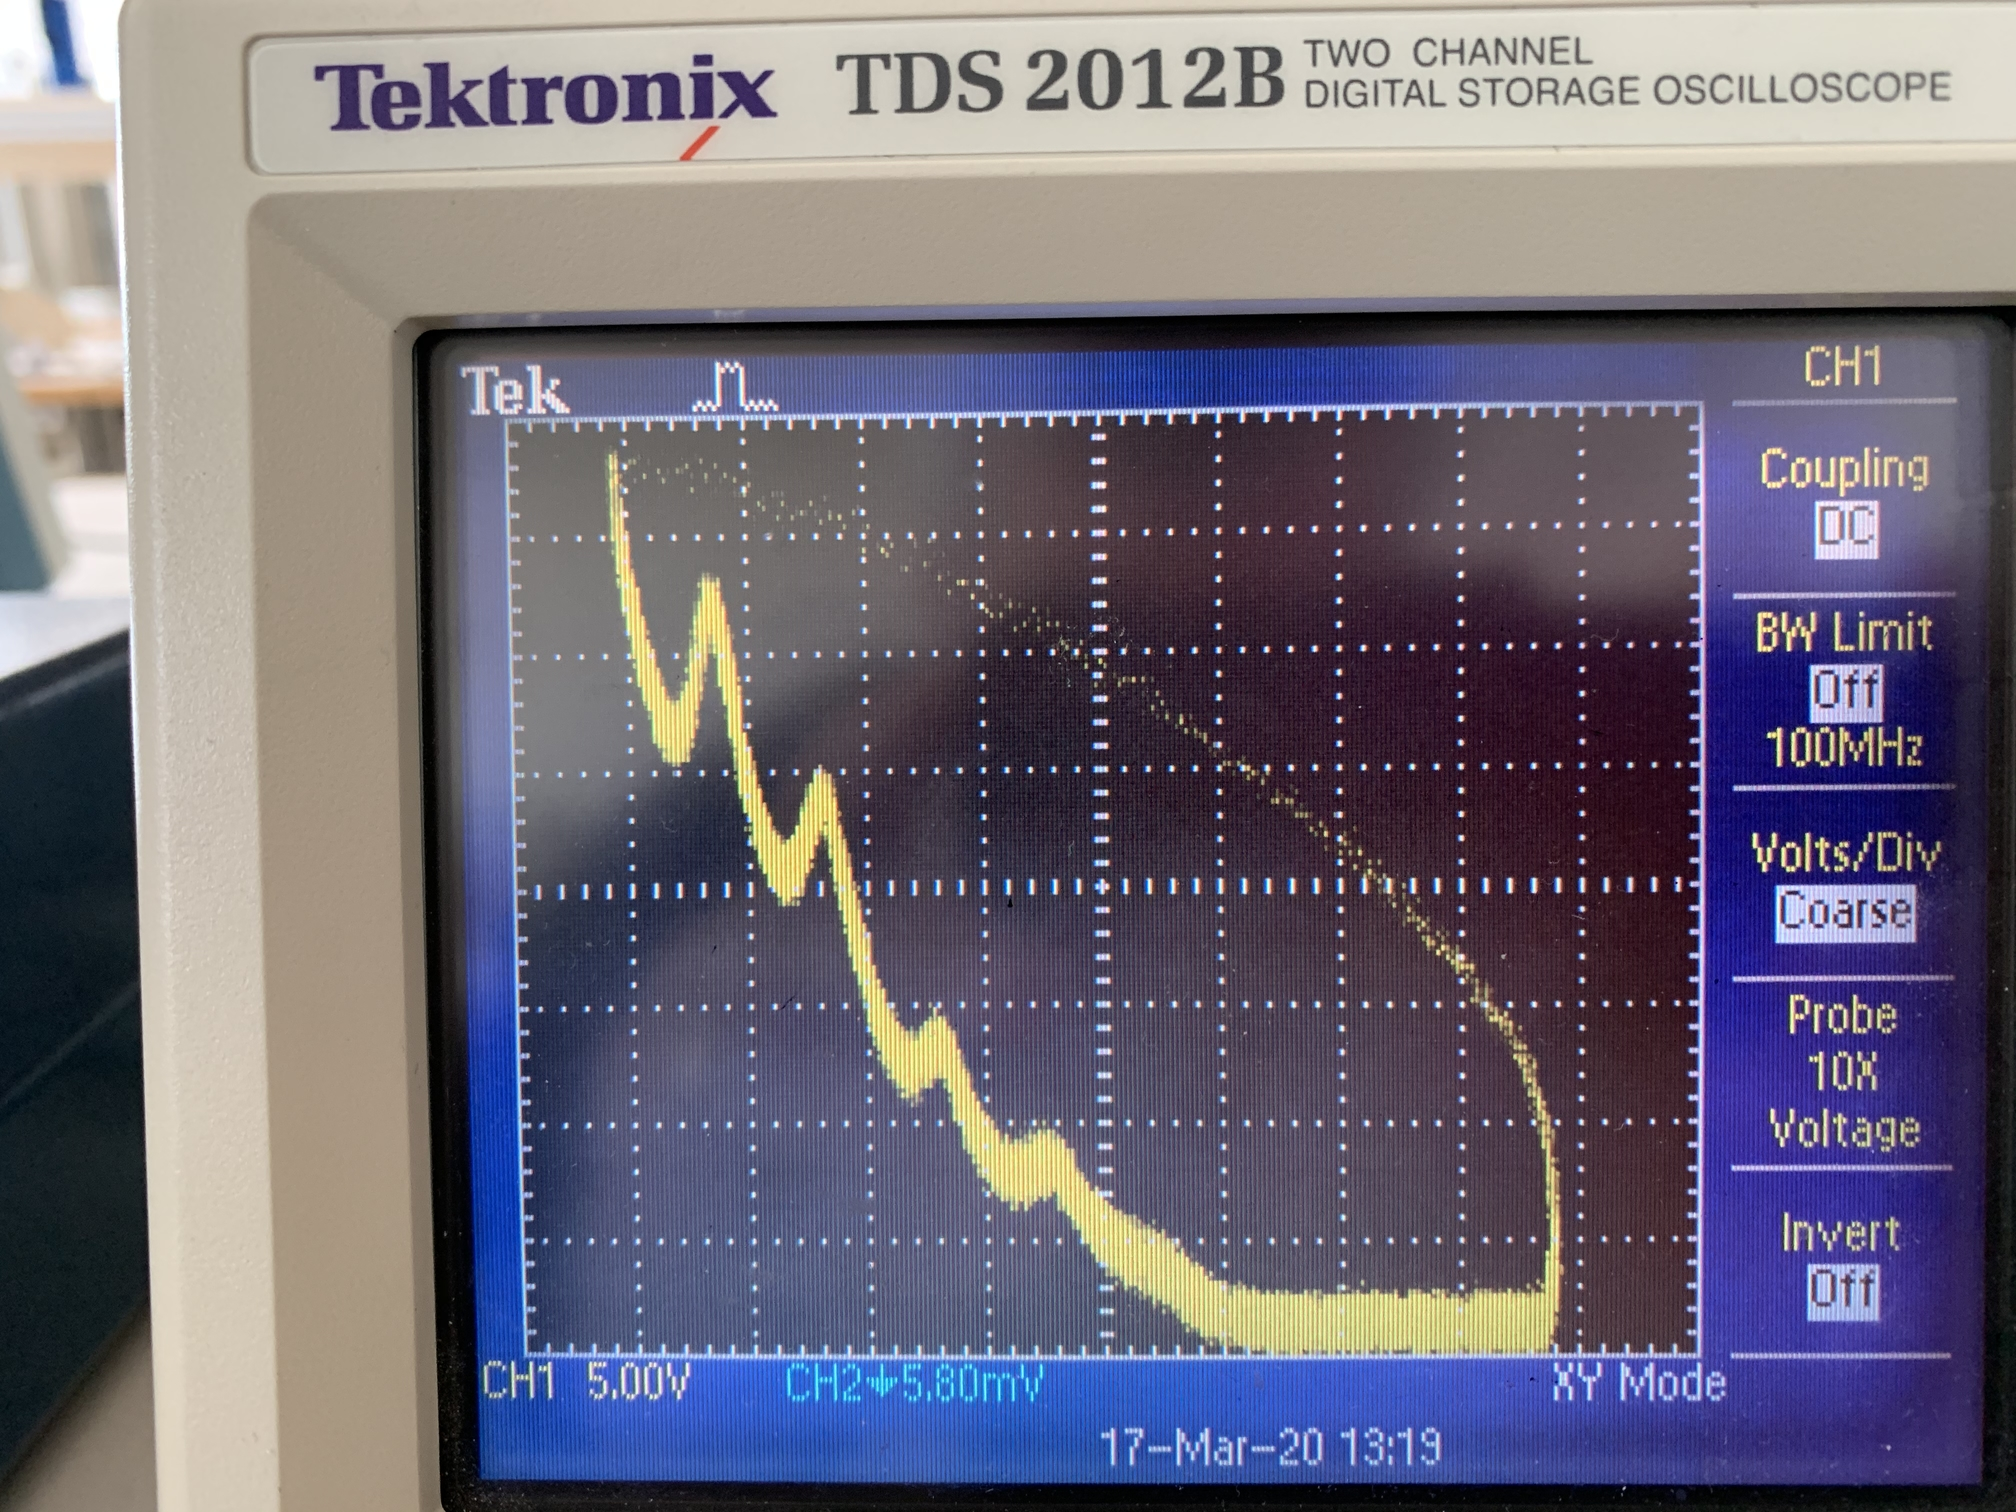
\includegraphics[width=10cm]{T=140_max_napetost.jpg}
    \caption{Prikaz spreminjanja $U_2$ in $U_{sig}$ na osciloskopu, 140 °C}
\end{figure}
Na x osi imamo prikazano negativno napetost $U_1$ na y osi pa je prikazana napetost signala $U_{sig}=\eta I_2 R.$

Če ponovno naredimo tabelo: 
\begin{table}[h]
	\centering
	\begin{tabular}{|c|c|c|c|c|c|}
		\hline
		
		Številka vrha & $U_1$ & $U_2$& $\Delta U = U_{n}- U_{n-1}$ [V] & $\Delta E= e_0\Delta U $ [eV] & $\overline{\Delta E}$\\
		\hline
		\hline
		1 & 0 & 38 & 0 & 0 & //\\
		\hline
		2 & 3.8 & 33 & 3.8 & 3.8 &// \\
		\hline
		3 & 8.2 & 25 & 4.4 & 4.4 & //\\
		\hline
		4 & 13.2 & 14 & 5 & 5 & //\\
		\hline
		5 & 17.8 & 9 & 4.6 & 4.6 &//\\
		\hline
		//& //& //&// & $4.667 eV \pm 0.25 eV$\\ 
		\hline
		\hline
	\end{tabular}
	\caption{Podatki o vrhovih na naši sliki 3.}		\label{140 °C}
\end{table}
Kometar k tabeli. Prve vrednosti nismo šteli v povprečje, saj je bil to odmik od začetka grafa, oz od začetka prikaza osciloskopa. \\
Vidimo, da je povprečje enako: 

$$\overline{\Delta E}=4.667 eV \pm 0.25 eV$$

Za napako smo ocelili, da je kar 0.25 eV, saj se pojavi zgolj zaradi našega nenatančnega odčitavanja iz grafa.

\pagebreak
\subsection{Temperatura 120 °C, ustrezna napetost}
Pri temperaturi 120 °C naredimo sliko na osciloskopu in jo nato obdelujemo. Slika je: 

\begin{figure}[H]
    \centering
    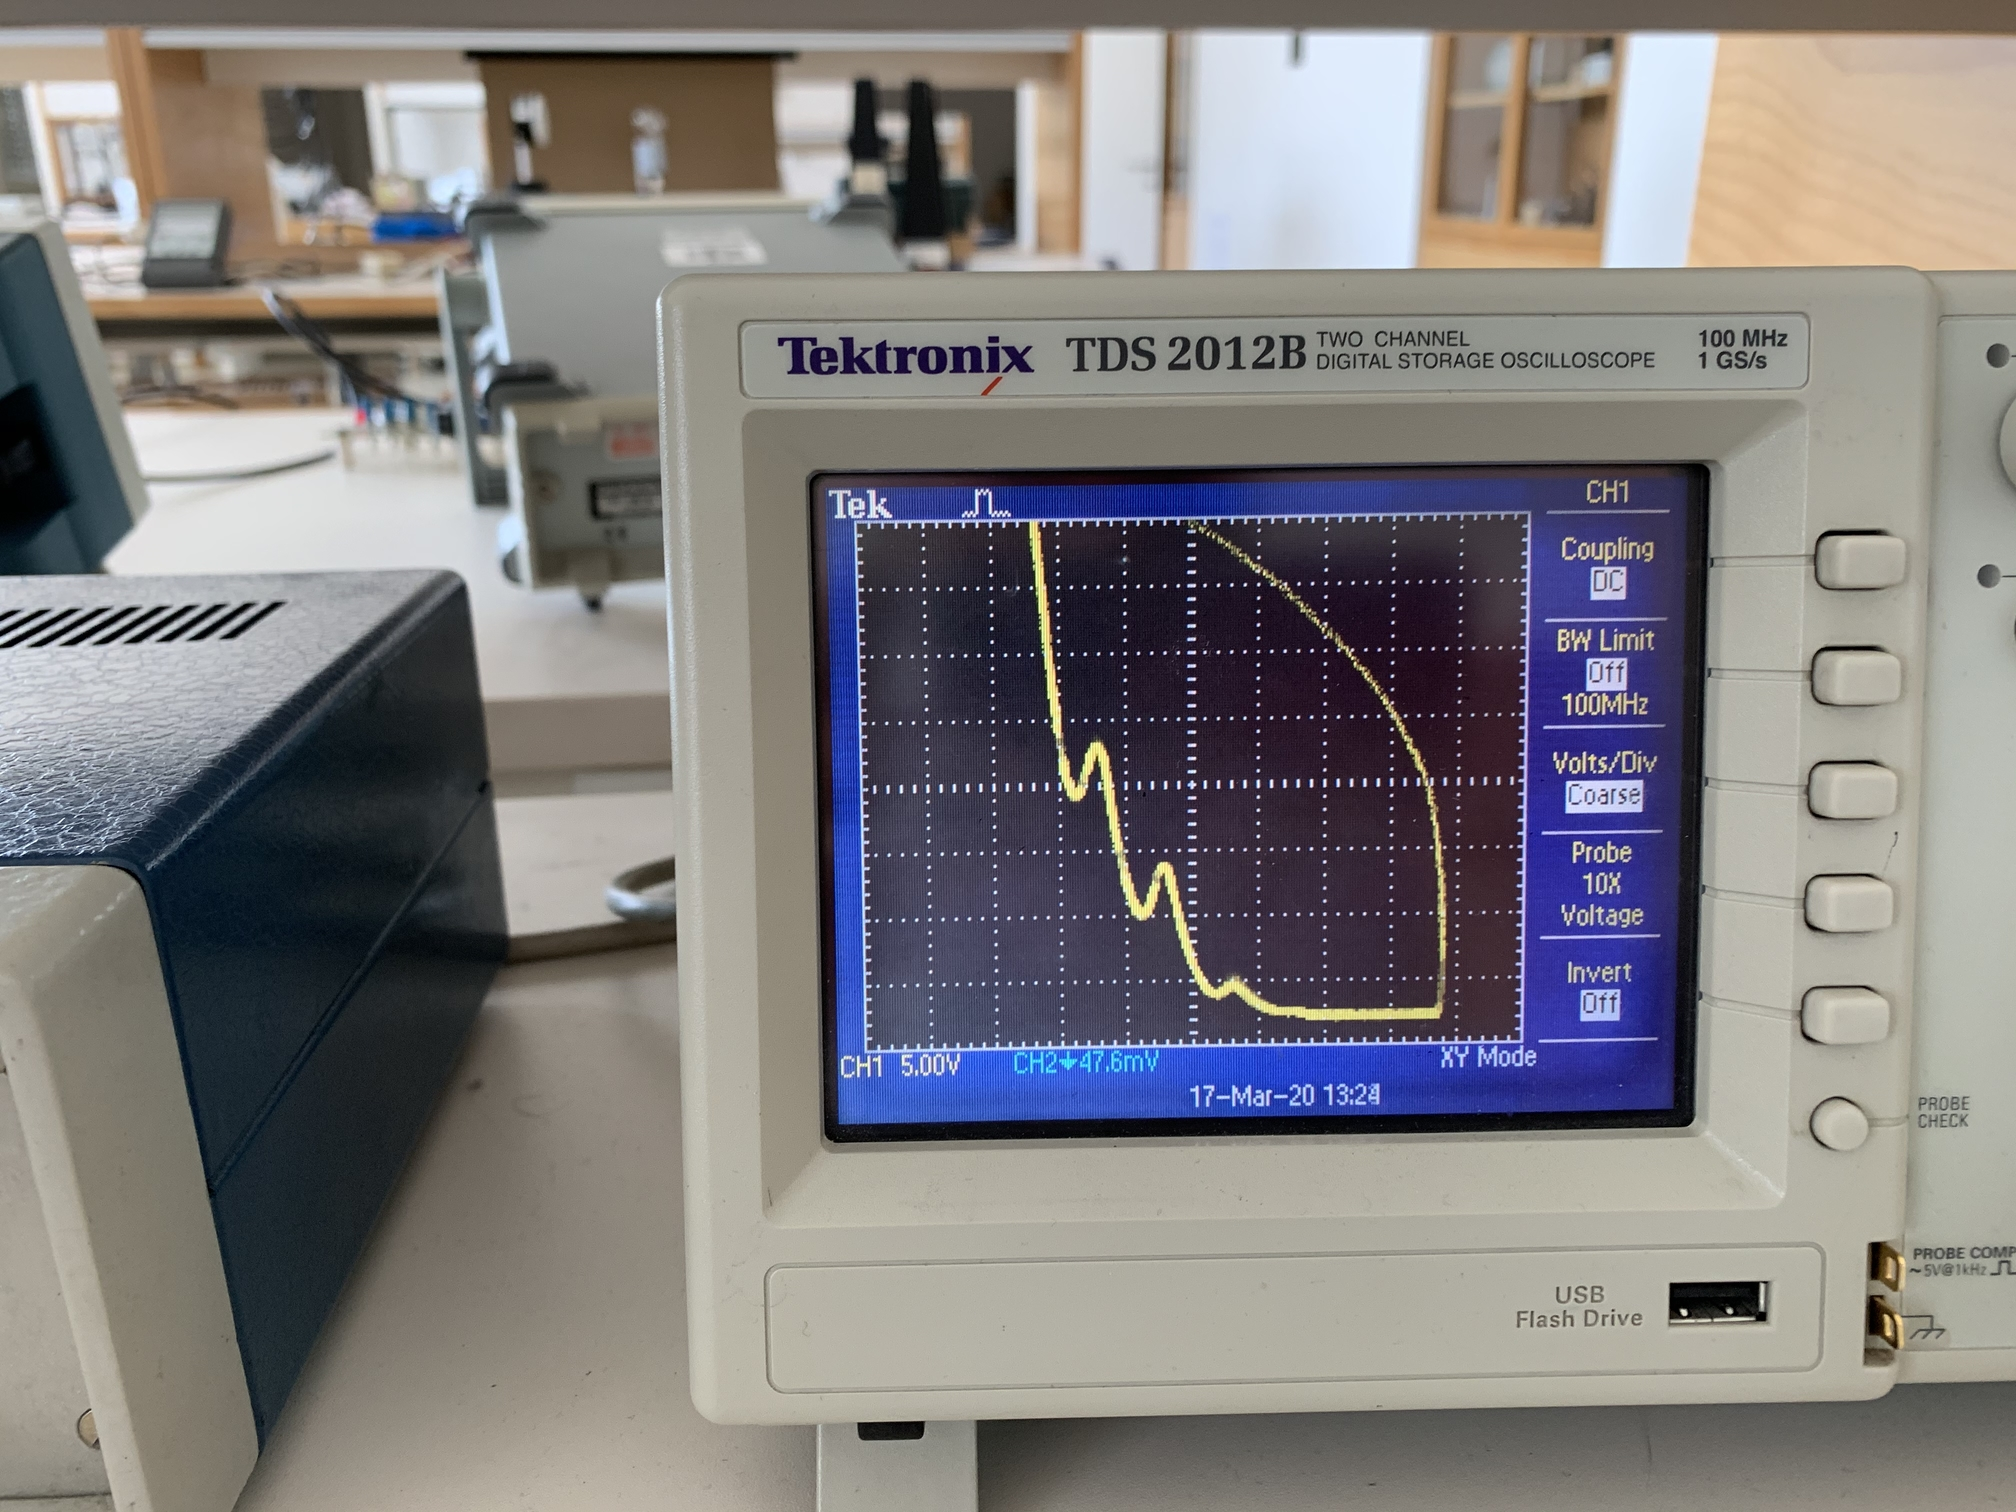
\includegraphics[width=10cm]{T=120_ustrezna_napetost.jpg}
    \caption{Prikaz spreminjanja $U_2$ in $U_{sig}$ na osciloskopu, 120 °C}
\end{figure}
Na x osi imamo prikazano negativno napetost $U_1$ na y osi pa je prikazana napetost signala $U_{sig}=\eta I_2 R.$

Če ponovno naredimo tabelo: 
\begin{table}[h]
	\centering
	\begin{tabular}{|c|c|c|c|c|c|}
		\hline
		
		Številka vrha & $U_1$ & $U_2$ & $\Delta U = U_{n}- U_{n-1}$ [V] & $\Delta E= e_0\Delta U $ [eV] & $\overline{\Delta E}$\\
		\hline
		\hline
		1 & 0 & 0 & 0 & //\\
		\hline
		2 & 3.2 & 24 & 3.2 & 3.2 &// \\
		\hline
		3 & 8.2 & 14 & 5 & 5 & //\\
		\hline
		4 & 13.2 & 5 & 5 & 5 & //\\
		\hline
		5 & 18.0 & 2 & 4.8 & 4.8 &//\\
		\hline
		//& //& //&// & $4.933 eV \pm 0.25 eV$\\ 
		\hline
		\hline
	\end{tabular}
	\caption{Podatki o vrhovih na naši sliki 3.}		\label{120 °C}
\end{table}
Kometar k tabeli. Prve vrednosti nismo šteli v povprečje, saj je bil to odmik od začetka grafa, oz od začetka prikaza osciloskopa. \\
Vidimo, da je povprečje enako: 

$$\overline{\Delta E}=4.933 eV \pm 0.25 eV$$

Za napako smo ocelili, da je kar 0.25 eV, saj se pojavi zgolj zaradi našega nenatančnega odčitavanja iz grafa.

\pagebreak
\subsection{Temperatura 120 °C, prevelika napetost}
Pri temperaturi 120 °C naredimo sliko na osciloskopu in jo nato obdelujemo, s spremembo, da smo tokrat nastavili prevelko napetost. To pomeni, da se je v naši celici ustvarila plazma, saj smo uspeli ionizirati atome Hg, ki nam nato spremeni meritve. Slika je: 

\begin{figure}[H]
    \centering
    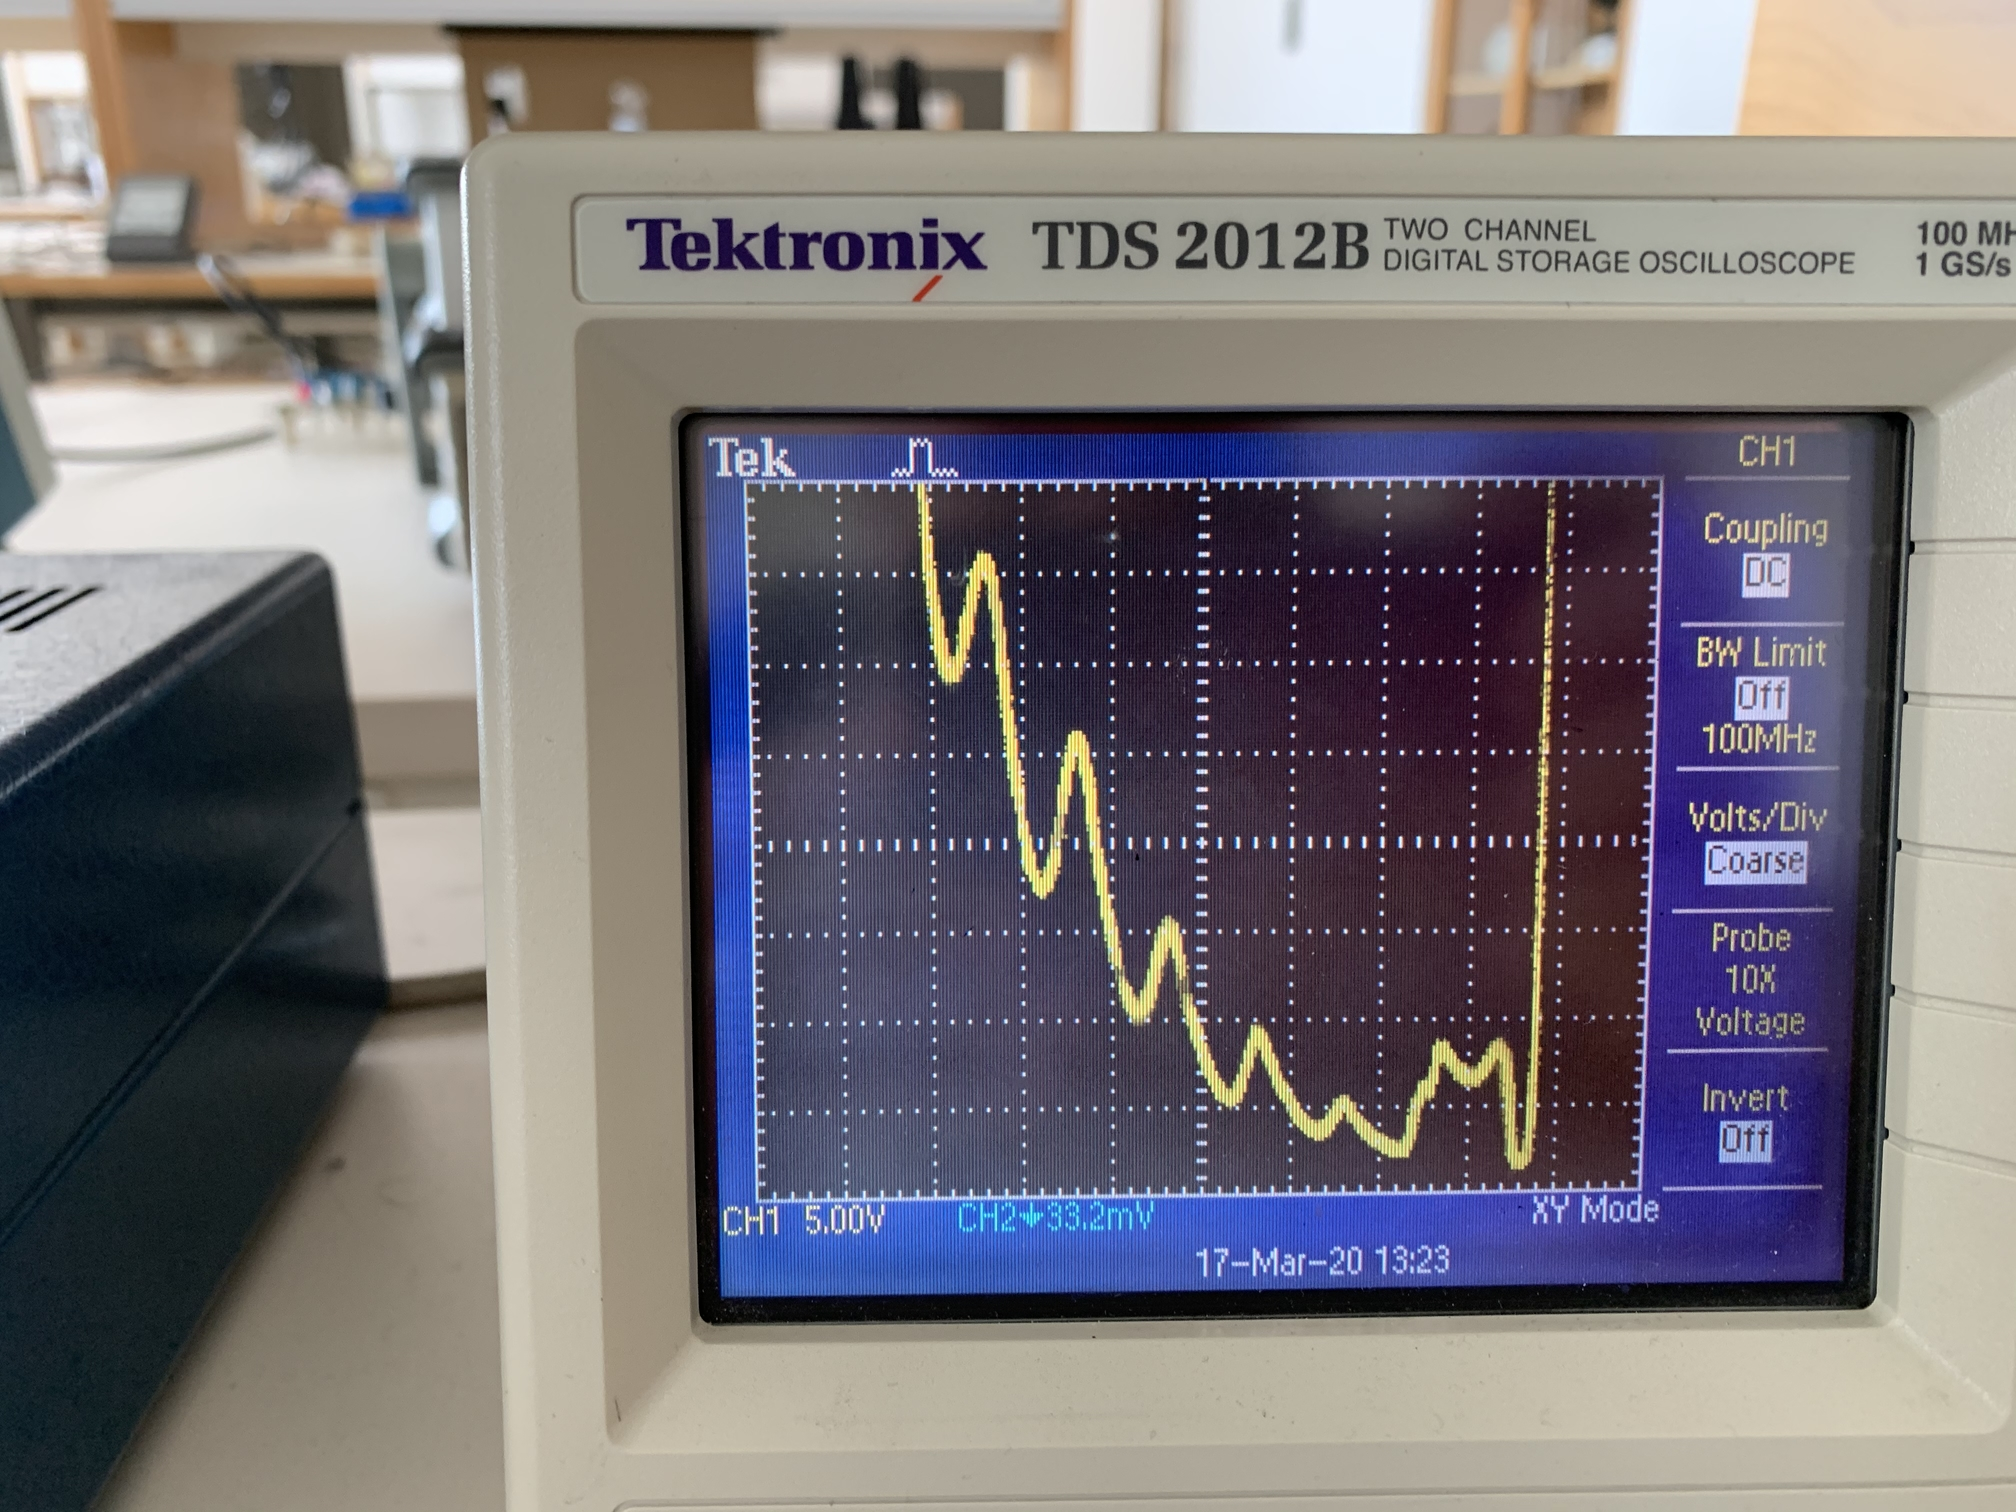
\includegraphics[width=10cm]{T=120_prevelika_napetost.jpg}
    \caption{Prikaz spreminjanja $U_2$ in $U_{sig}$ na osciloskopu, 120 °C}
\end{figure}
Na x osi imamo prikazano negativno napetost $U_1$ na y osi pa je prikazana napetost signala $U_{sig}=\eta I_2 R.$

Če ponovno naredimo tabelo: 
\begin{table}[h]
	\centering
	\begin{tabular}{|c|c|c|c|c|}
		\hline
		
		Številka vrha & $U_1$ & $\Delta U = U_{n}- U_{n-1}$ [V] & $\Delta E= e_0\Delta U $ [eV] & $\overline{\Delta E}$\\
		\hline
		\hline
		1 & 0 & 0 & 0 & //\\
		\hline
		2 & 3.2 & 3.2 & 3.2 &// \\
		\hline
		3 & 8.2 & 5 & 5 & //\\
		\hline
		4 & 13.2 & 5 & 5 & //\\
		\hline
		5 & 18.1 & 4.9 & 4.9 &//\\
		\hline
		6 & 23 & 4.9 & 4.9 &//\\
		\hline
		7 & 28.3 & 5.3 & 5.3 &//\\
		\hline
		//& //& //&// & $5.02 eV \pm 0.25 eV$\\ 
		\hline
		\hline
	\end{tabular}
	\caption{Podatki o vrhovih na naši sliki 3.}		\label{120 °C}
\end{table}
Kometar k tabeli. Prve vrednosti nismo šteli v povprečje, saj je bil to odmik od začetka grafa, oz od začetka prikaza osciloskopa. \\
Vidimo, da je povprečje enako: 

$$\overline{\Delta E}=5.02 eV \pm 0.25 eV$$

Za napako smo ocelili, da je kar 0.25 eV, saj se pojavi zgolj zaradi našega nenatančnega odčitavanja iz grafa.

\subsection{Temperatura 26 °C}
Pri temperaturi 26 °C, kar je temperatura ozračja naredimo sliko na osciloskopu in jo nato obdelujemo. Slika je: 

\begin{figure}[H]
    \centering
    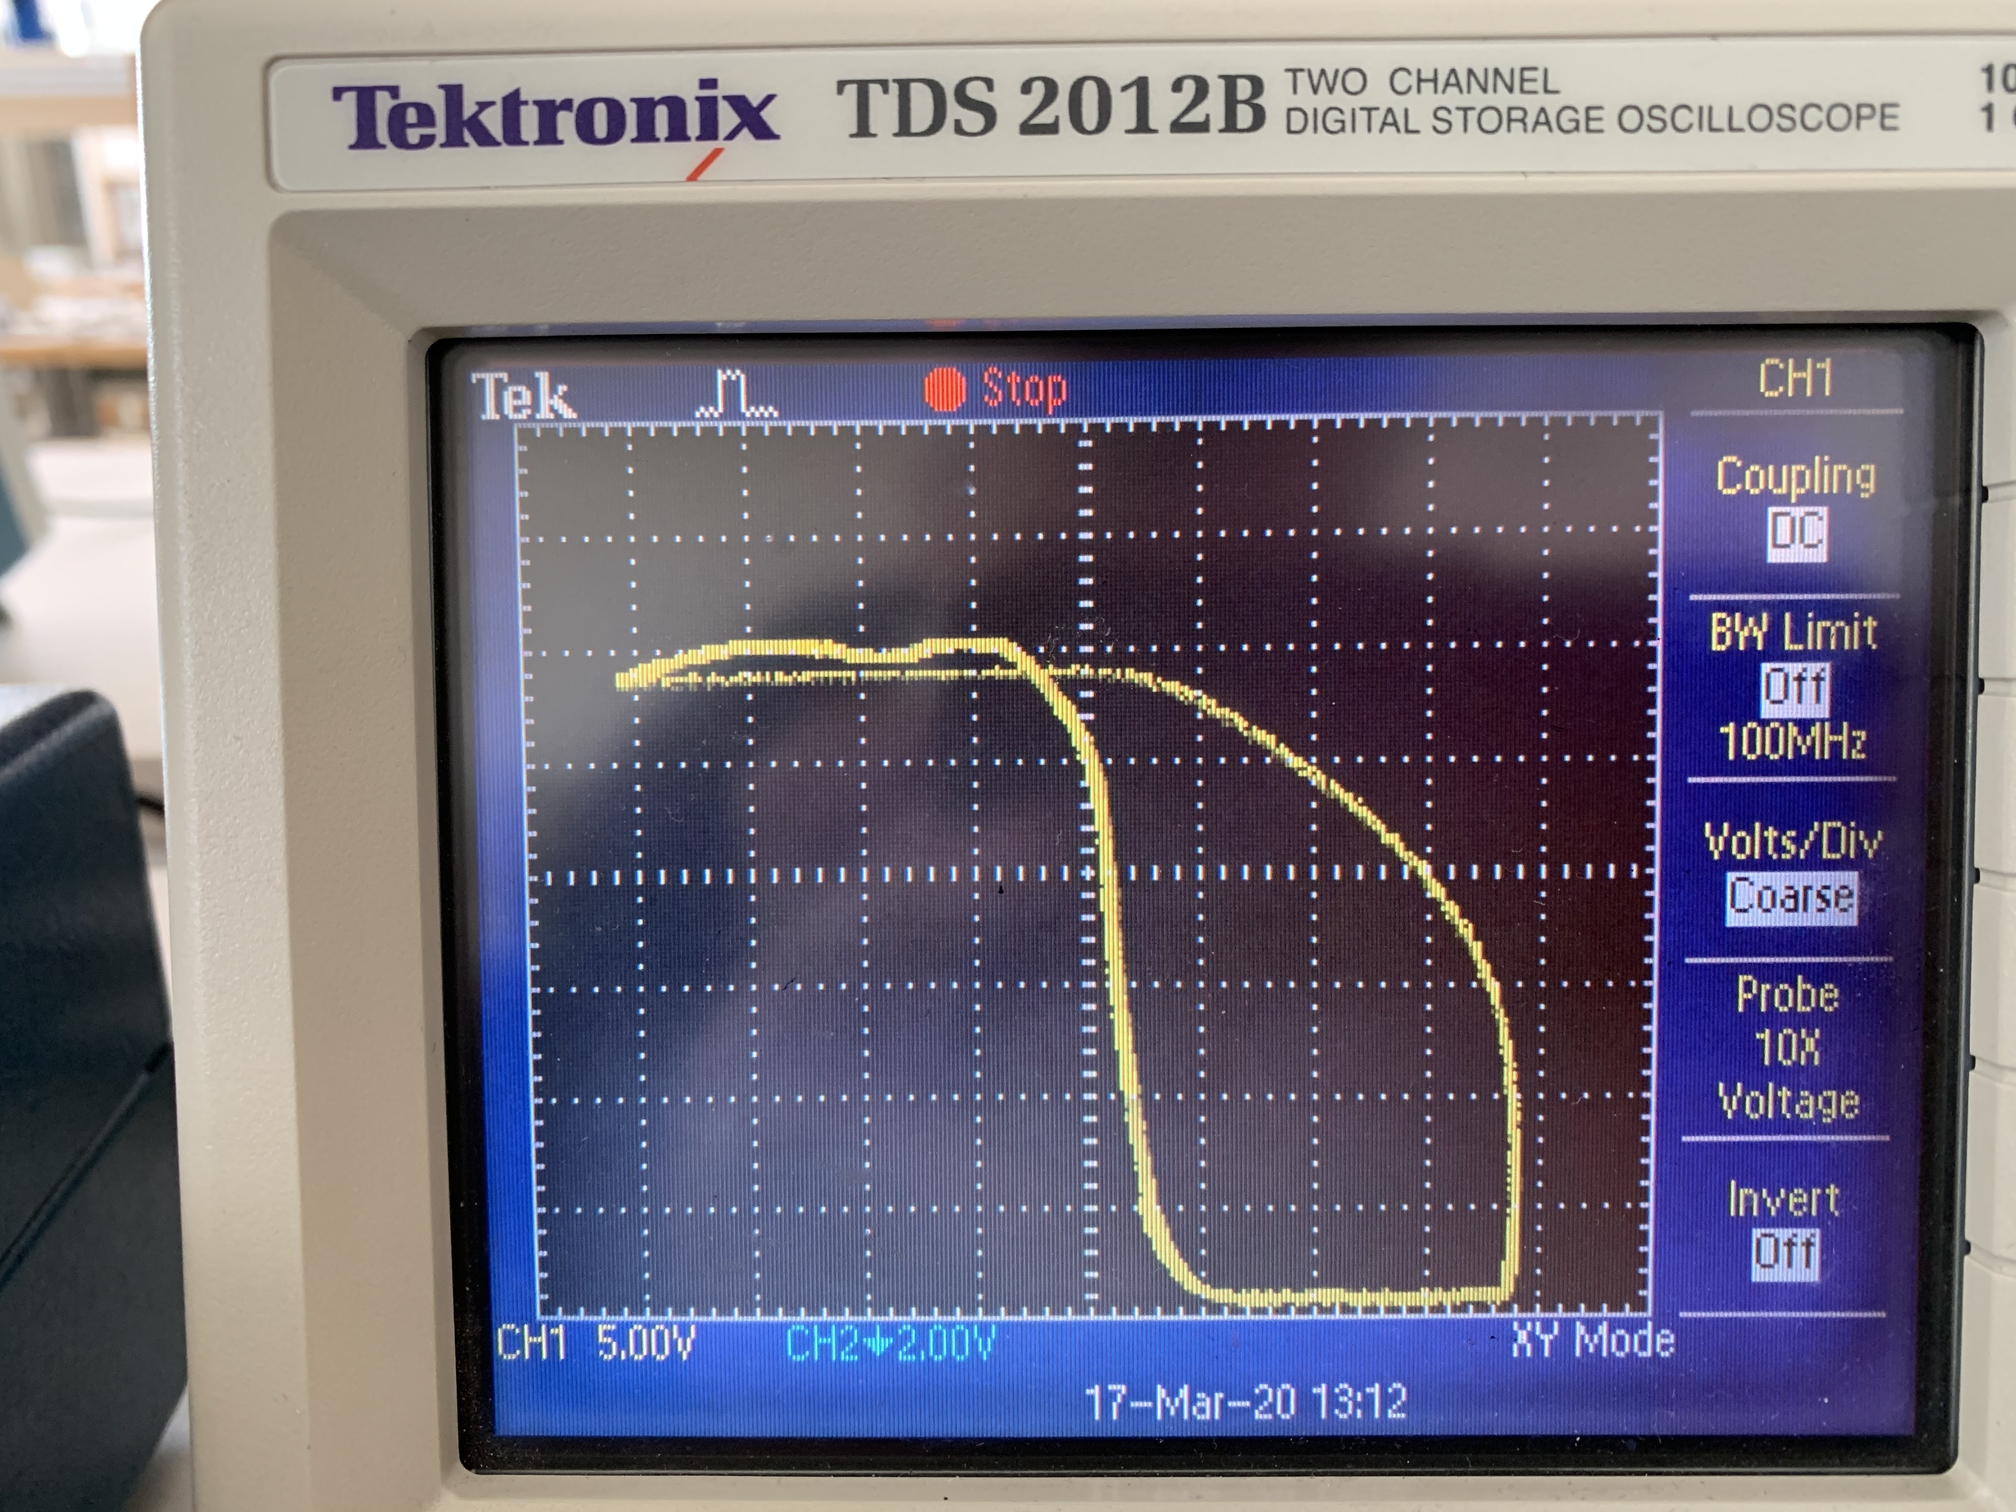
\includegraphics[width=10cm]{T=26C_max_napetost.jpg}
    \caption{Prikaz spreminjanja $U_2$ in $U_{sig}$ na osciloskopu, 26 °C}
\end{figure}
Na x osi imamo prikazano negativno napetost $U_1$ na y osi pa je prikazana napetost signala $U_{sig}=\eta I_2 R.$
Vidimo, da je, če uporabimo maksimalno napetost popolnoma nerazvidno, kje pride do prehoda, zato uporabimo neko srednjo napetost in poglejmo, kaj dobimo:
\begin{figure}[H]
    \centering
    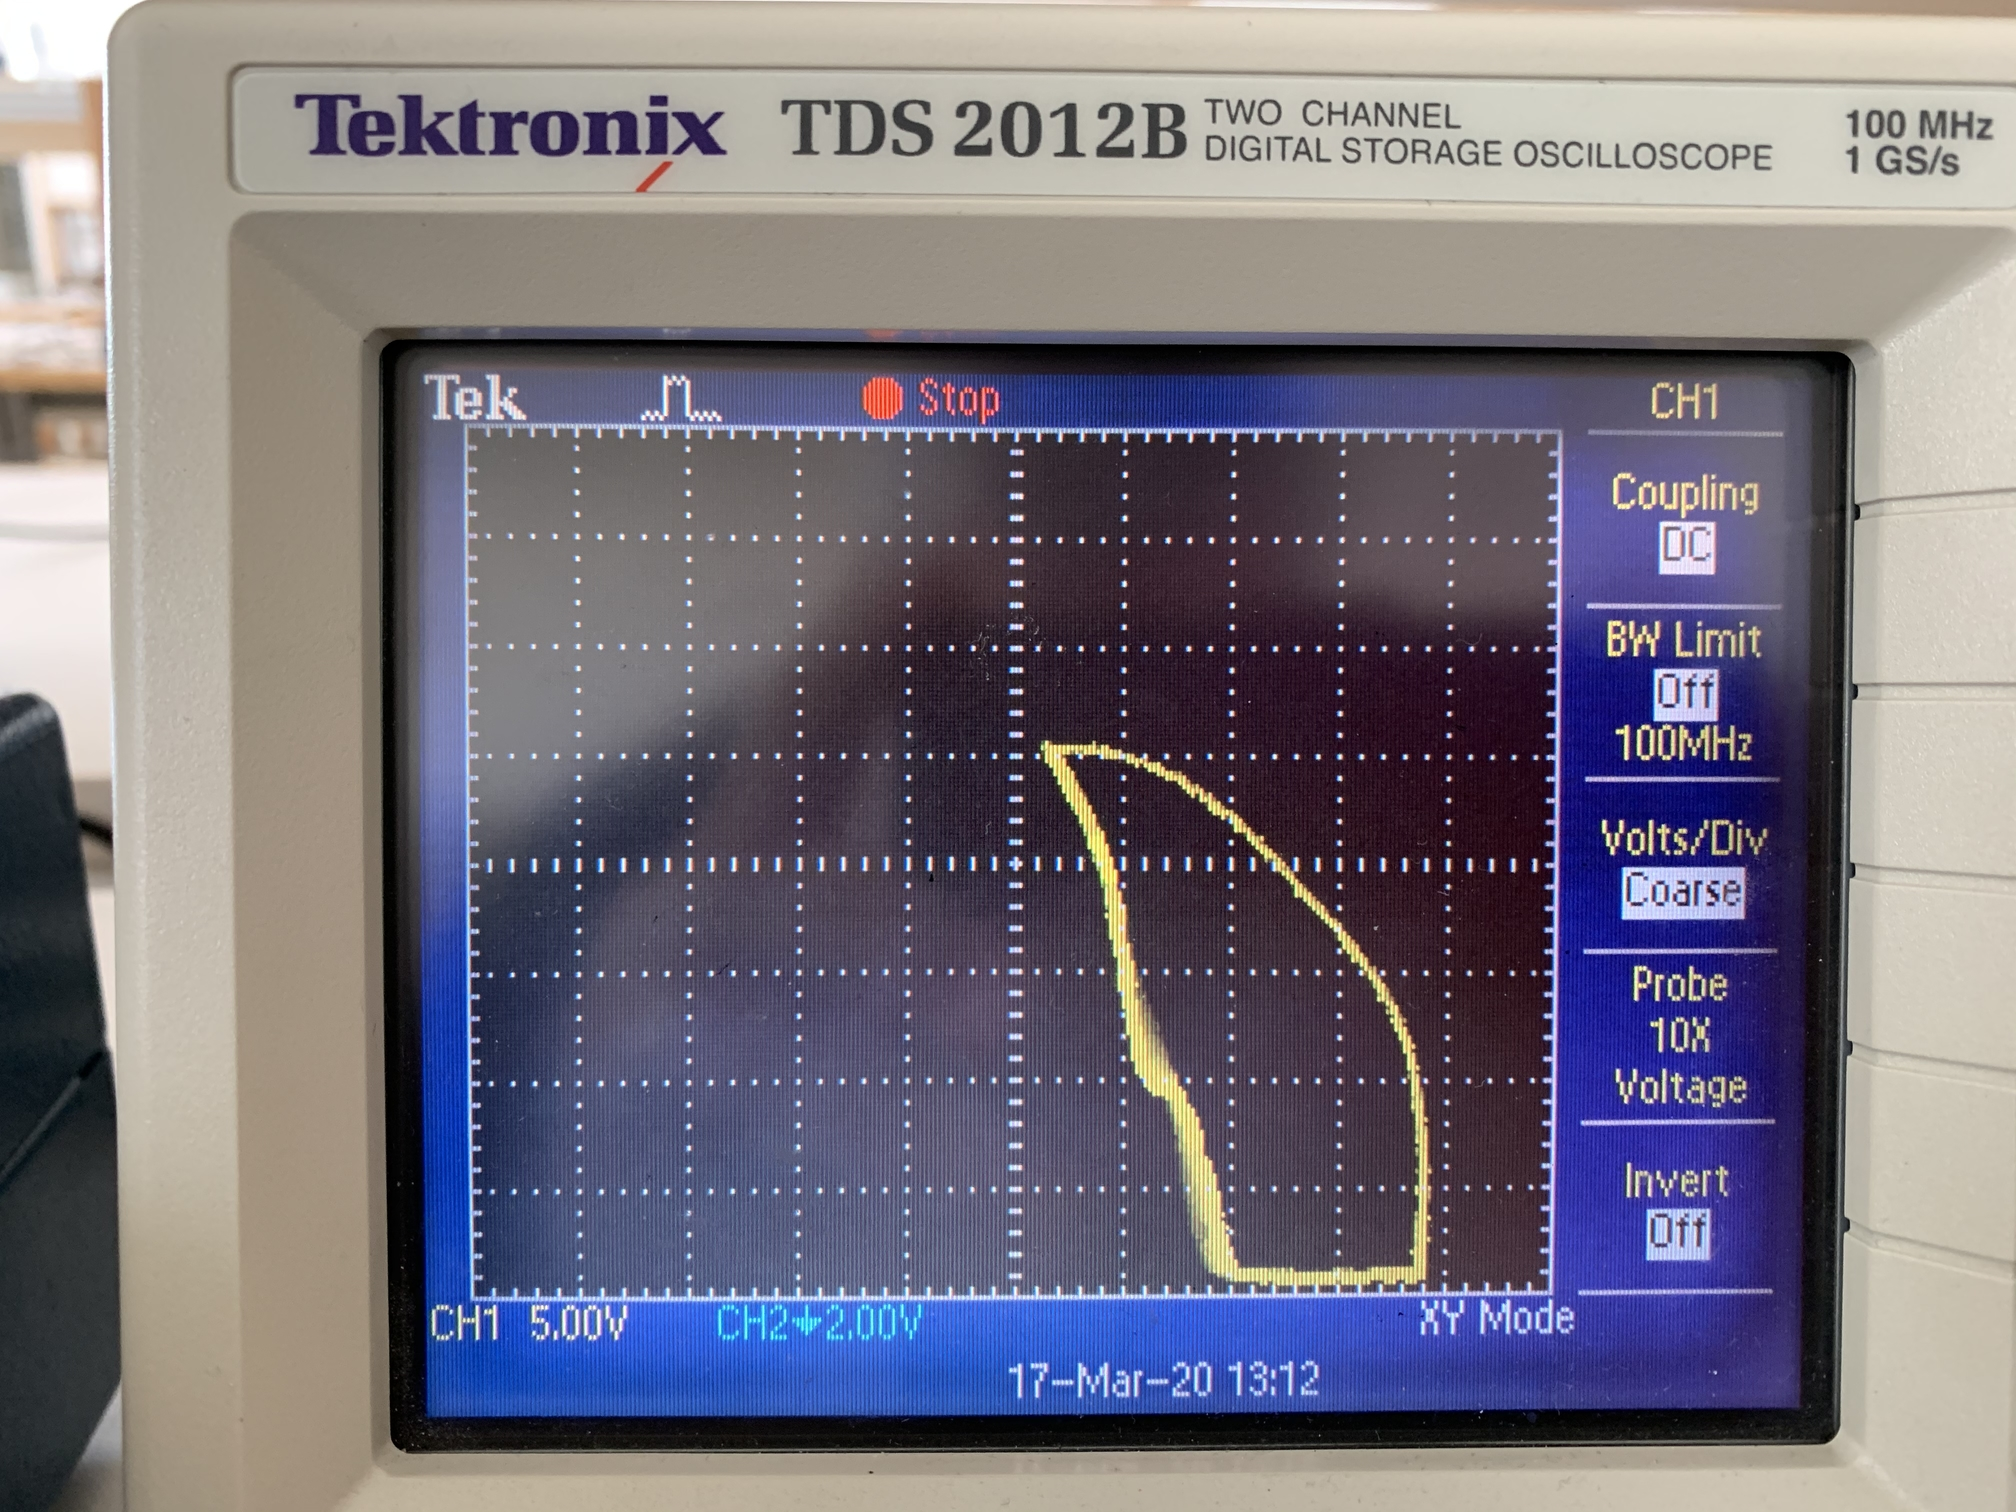
\includegraphics[width=10cm]{T=26C_srednja_napetost.jpg}
    \caption{Prikaz spreminjanja $U_2$ in $U_{sig}$ na osciloskopu, 26 °C}
\end{figure}

Še vedno ni popolne razvidnosti, ampak z malo truda lahko vidimo, kje se zgodi prehod.

Če ponovno naredimo tabelo: 
\begin{table}[H]
	\centering
	\begin{tabular}{|c|c|c|c|c|}
		\hline
		
		Številka vrha & $U_1$ & $\Delta U = U_{n}- U_{n-1}$ [V] & $\Delta E= e_0\Delta U $ [eV] & $\overline{\Delta E}$\\
		\hline
		\hline
		1 & 0 & 0 & 0 & //\\
		\hline
		2 & 3.5 & 3.5 & 3.5 & // \\
		\hline
		//& //& //&// & $3.5 eV \pm 0.25 eV$\\ 
		\hline
		\hline
	\end{tabular}
	\caption{Podatki o vrhovih na naši sliki 3.}		\label{26 °C}
\end{table}
Kometar k tabeli. Prve vrednosti nismo šteli v povprečje, saj je bil to odmik od začetka grafa, oz od začetka prikaza osciloskopa. \\
Vidimo, da je povprečje enako: 

$$\overline{\Delta E}=3.5 eV \pm 0.25 eV$$

Za napako smo ocelili, da je kar 0.25 eV, saj se pojavi zgolj zaradi našega nenatančnega odčitavanja iz grafa.
Vidimo, da nam ta vrednost ne bo kaj dosti koristila, saj je bilo popolnoma nerazvidno, kje se pojavi naš vrh. 

\subsection{Skupna $\Delta E$}
Če sedaj pogledamo povprečje naših vseh zbranih meritev za $\Delta E$ vidimo, da dobimo:

\begin{table}[H]
	\centering
	\begin{tabular}{|c|c|c|}
		\hline
		Temperatura  &  $\Delta E= e_0\Delta U $ [eV] & $\overline{\Delta E}$\\
		\hline
		\hline
		180  & 4.56 & //\\
		\hline
		160  & 4.725 & //\\
		\hline
		140  & 4.667 & //\\
		\hline
		120 normal  & 4.933 & //\\
		\hline
		120 max  & 5.02 & //\\
		\hline
		//&  // & $4.78 eV \pm 0.25 eV$\\ 
		\hline
		\hline
	\end{tabular}
	\caption{Podatki o vrhovih na naši sliki 3.}	
\end{table}
Dobimo da je povprečje vseh $\Delta E$ kar enako:

$$\overline{\Delta E}=4.78 eV \pm 0.25 eV$$

Kar lahko rečemo, da je razlika med prvim in drugim vzbujenim stanjem. 

\section{DODATEK; Odvisnost višine vrhov od temperature}
V dodatnih navodilih za vajo je priporočeno, da naredimo še odvisnost višine vrhov od temperature. Za to bomo ponovno sestavili tabelo, le da bomo tokrat za vsak vrh opazovali odvisnost toka od Napetosti. To smo navedli že v prvotnih tabelah in vidimo, da ni neke funckije ki bi napvedovala, kako pada. Vidimo pa lahko, da upada amplituda z manjšanjem temperature.


\end{document}